% This must be in the first 5 lines to tell arXiv to use pdfLaTeX, which is strongly recommended.
\pdfoutput=1
% In particular, the hyperref package requires pdfLaTeX in order to break URLs across lines.

\documentclass[11pt]{article}

% Change "review" to "final" to generate the final (sometimes called camera-ready) version.
% Change to "preprint" to generate a non-anonymous version with page numbers.

% TODO: change this to "final" before submission
\usepackage["preprint"]{acl}

% Standard package includes
\usepackage{times}
\usepackage{latexsym}

% For proper rendering and hyphenation of words containing Latin characters (including in bib files)
\usepackage[T1]{fontenc}
% For Vietnamese characters
% \usepackage[T5]{fontenc}
% See https://www.latex-project.org/help/documentation/encguide.pdf for other character sets

% This assumes your files are encoded as UTF8
\usepackage[utf8]{inputenc}

% This is not strictly necessary, and may be commented out,
% but it will improve the layout of the manuscript,
% and will typically save some space.
\usepackage{microtype}

% This is also not strictly necessary, and may be commented out.
% However, it will improve the aesthetics of text in
% the typewriter font.
\usepackage{inconsolata}

%Including images in your LaTeX document requires adding
%additional package(s)
\usepackage{graphicx}

\usepackage{todonotes}
\usepackage{booktabs}
\usepackage{multirow}
\usepackage{graphicx}
\usepackage{subcaption}
\usepackage[margin=1in]{geometry}



% If the title and author information does not fit in the area allocated, uncomment the following
%
%\setlength\titlebox{<dim>}
%
% and set <dim> to something 5cm or larger.

\title{Separate ONE-PEACE You Describe}

% Author information can be set in various styles:
% For several authors from the same institution:
% \author{Author 1 \and ... \and Author n \\
%         Address line \\ ... \\ Address line}
\author{Vincent La \quad Richard Wen \quad Sambit Sahoo \\
        University of Maryland, College Park}

% if the names do not fit well on one line use
%         Author 1 \\ {\bf Author 2} \\ ... \\ {\bf Author n} \\
% For authors from different institutions:
% \author{Author 1 \\ Address line \\  ... \\ Address line
%         \And  ... \And
%         Author n \\ Address line \\ ... \\ Address line}
% To start a separate ``row'' of authors use \AND, as in
% \author{Author 1 \\ Address line \\  ... \\ Address line
%         \AND
%         Author 2 \\ Address line \\ ... \\ Address line \And
%         Author 3 \\ Address line \\ ... \\ Address line}

% \author{First Author \\
%   Affiliation / Address line 1 \\
%   Affiliation / Address line 2 \\
%   Affiliation / Address line 3 \\
%   \texttt{email@domain} \\\And
%   Second Author \\
%   Affiliation / Address line 1 \\
%   Affiliation / Address line 2 \\
%   Affiliation / Address line 3 \\
%   \texttt{email@domain} \\}

%\author{
%  \textbf{First Author\textsuperscript{1}},
%  \textbf{Second Author\textsuperscript{1,2}},
%  \textbf{Third T. Author\textsuperscript{1}},
%  \textbf{Fourth Author\textsuperscript{1}},
%\\
%  \textbf{Fifth Author\textsuperscript{1,2}},
%  \textbf{Sixth Author\textsuperscript{1}},
%  \textbf{Seventh Author\textsuperscript{1}},
%  \textbf{Eighth Author \textsuperscript{1,2,3,4}},
%\\
%  \textbf{Ninth Author\textsuperscript{1}},
%  \textbf{Tenth Author\textsuperscript{1}},
%  \textbf{Eleventh E. Author\textsuperscript{1,2,3,4,5}},
%  \textbf{Twelfth Author\textsuperscript{1}},
%\\
%  \textbf{Thirteenth Author\textsuperscript{3}},
%  \textbf{Fourteenth F. Author\textsuperscript{2,4}},
%  \textbf{Fifteenth Author\textsuperscript{1}},
%  \textbf{Sixteenth Author\textsuperscript{1}},
%\\
%  \textbf{Seventeenth S. Author\textsuperscript{4,5}},
%  \textbf{Eighteenth Author\textsuperscript{3,4}},
%  \textbf{Nineteenth N. Author\textsuperscript{2,5}},
%  \textbf{Twentieth Author\textsuperscript{1}}
%\\
%\\
%  \textsuperscript{1}Affiliation 1,
%  \textsuperscript{2}Affiliation 2,
%  \textsuperscript{3}Affiliation 3,
%  \textsuperscript{4}Affiliation 4,
%  \textsuperscript{5}Affiliation 5
%\\
%  \small{
%    \textbf{Correspondence:} \href{mailto:email@domain}{email@domain}
%  }
%}

\begin{document}
\maketitle
\begin{abstract}
\todo{idk if people include citations in the abstract but i have the mains one included for now -Vincent}

Language-queried audio source separation (LASS) is the task of isolating arbitrary sounds using a natural language description of the desired source. We modify AudioSep \cite{audiosep}, a LASS architecture, by replacing the QueryNet with ONE-PEACE \cite{onepeace}, which is a general representation model for aligning vision, audio, language, and potentially unlimited modalities. The original AudioSep architecture is used as a baseline comparison, where CLAP is used as the QueryNet. We find that ONE-PEACE only performs comparably on LASS, despite significantly outperforming CLAP on other downstream audio-language tasks like retrieval.


% It has significantly more parameters than CLAP, includes alignments for visual data (and potentially more modalities), and outperforms CLAP on text to audio retrieval tasks.
\end{abstract}

\section{Introduction}
Performance on multi-modal downstream tasks has significantly improved in recent years as representation models that align different modalities have become more popular. These representation models seek to encode different types of input into a shared embedding space where similar concepts across different modalities are close to each other. In the audio-language domain, Contrastive Language-Audio Pretraining (CLAP) \cite{clap} has emerged as a prominent model for a variety of tasks.

One particular downstream audio-language task where CLAP has been used is Language-queried audio source separation (LASS) \cite{lass}. LASS is the task of isolating arbitrary sounds using a natural language description of the desired source. Given some input audio with multiple sources of sound, the goal is to mask out audio sources that are unrelated to the language query. The alignment between audio and language modalities in the CLAP embedding space is 
\todo[inline]{smth about how modality alignment in shared embedding space is important for LASS --> tie into ONE-PEACE --> compare retrieval performance to argue that ONE-PEACE generally has the better alignment}

\section{Related Work}

\subsection{Language-Queried Audio Source Separation}
Language-Queried Audio Source Separation (LASS) achieves the task of separating arbitrary sound sources using natural language descriptions of the desired source. The language query is passed to the QueryNet, which encodes the query into an embedding space. Generally, within this embedding space, audio and language modalities are aligned. A Short-time Fourier transform is applied to the input mixture waveform, which converts the raw audio data into a spectrogram representing the evolution of the signal’s frequency content over time. Both of the resulting representations are then sent to SeparationNet, which uses the embedded language query to determine the frequencies of the audio data to preserve and cut. The embedded language query is incorporated into the SeparationNet via Feature-wise Linearly modulated (FiLm) layers. The FiLm layers are small fully-connected networks that learn modulation parameters that are applied per feature map, to contextualize the SeparationNet hidden representations with the language query. Finally, the output frequencies are put into an inverse STFT to convert them back to raw audio data. 

\todo[inline]{CITE: https://arxiv.org/pdf/2206.04769}
\subsection{Contrastive Language-Audio Pretraining}
Contrastive Language-Audio Pretraining (CLAP) is an approach that learns to connect natural language and audio modalities. Using two encoders and contrastive learning, a multimodal joint space can be created with audio and text descriptions. The audio encoder is used to process audio data and the text encoder handles natural language text queries. These encoders are trained simultaneously using contrastive learning, which maximizes the similarity of aligned audio-text pairs in a shared embedding space while minimizing the similarity of unaligned pairs. CLAP utilizes a symmetric cross-entropy loss over a similarity matrix to optimize the audio and text encoders. The loss function ensures that the embeddings of aligned audio-text pairs are close in the embedding space, while unaligned pairs are further apart. In testing, the audio encoder generates embeddings for audio inputs and the text encoder produces embeddings for text queries to compare in the embedding space. CLAP has an embedding dimension size of 512.

\subsection{ONE-PEACE}

The embedding dimension size of ONE-PEACE is 1536, three times larger than CLAP.

\section{Methods}
\subsection{LASS Baseline Approach}
\subsection{ONE-PEACE LASS}
% (16k Hz, window size 1024, hop size 160)
We used the baseline model from the DCASE 2024 Task 9 challenge \todo{how to cite DCASE workshop?}, which is a scaled-down version of the full AudioSep model. 

\todo[inline]{CLAP model is using HTSAT and Roberta as base models, ONE-PEACE trained from scratch without pretrained initializations}

\section{Results}
\documentclass{article}
\usepackage{graphicx}
\usepackage{subcaption}
\usepackage[margin=1in]{geometry}


% Visual Spectrograms
\begin{figure*}[htbp]
    \centering
    % Row 1 Best One-PEACE SDR
    \begin{subfigure}[b]{0.185\textwidth}
        \centering
        \scriptsize\textbf{"The heart is beating forcefully, making a thumping sound"}
        \vspace{5.0mm}
    \end{subfigure}
    \begin{subfigure}[b]{0.185\textwidth}
        \centering
        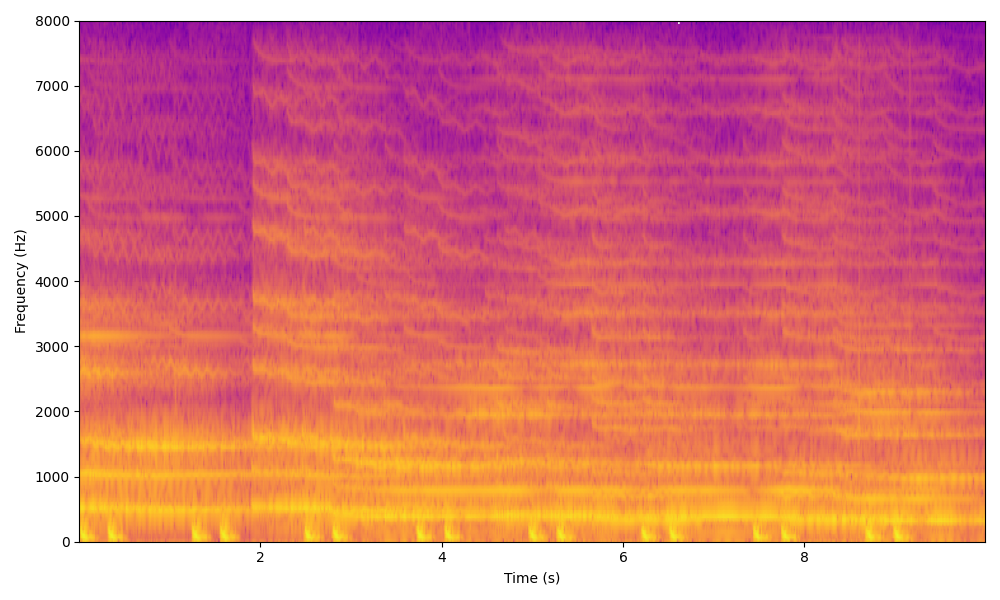
\includegraphics[width=\textwidth]{plots/onepeace_best_sdr/onepeace mixture_spectrogram.png}
    \end{subfigure}
    \begin{subfigure}[b]{0.185\textwidth}
        \centering
        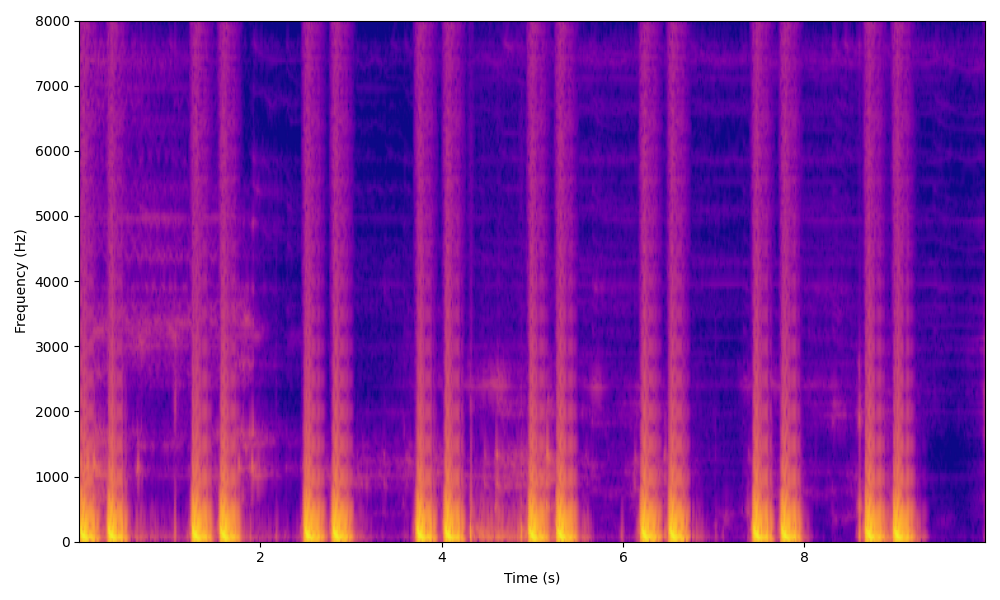
\includegraphics[width=\textwidth]{plots/onepeace_best_sdr/onepeace sep_spectrogram.png}
    \end{subfigure}
    \begin{subfigure}[b]{0.185\textwidth}
        \centering
        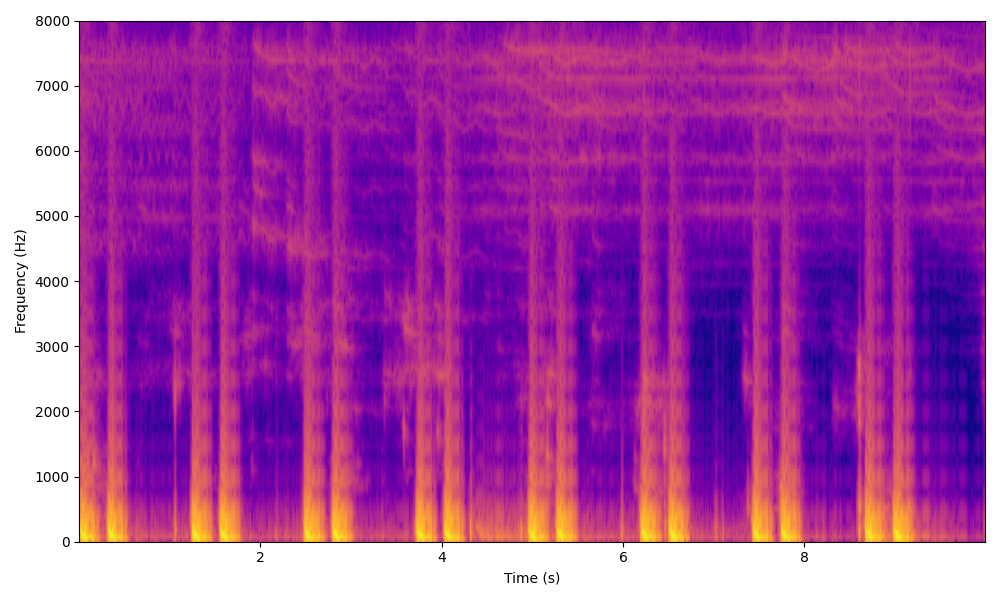
\includegraphics[width=\textwidth]{plots/onepeace_best_sdr/clap sep_spectrogram.png}
    \end{subfigure}
    \begin{subfigure}[b]{0.185\textwidth}
        \centering
        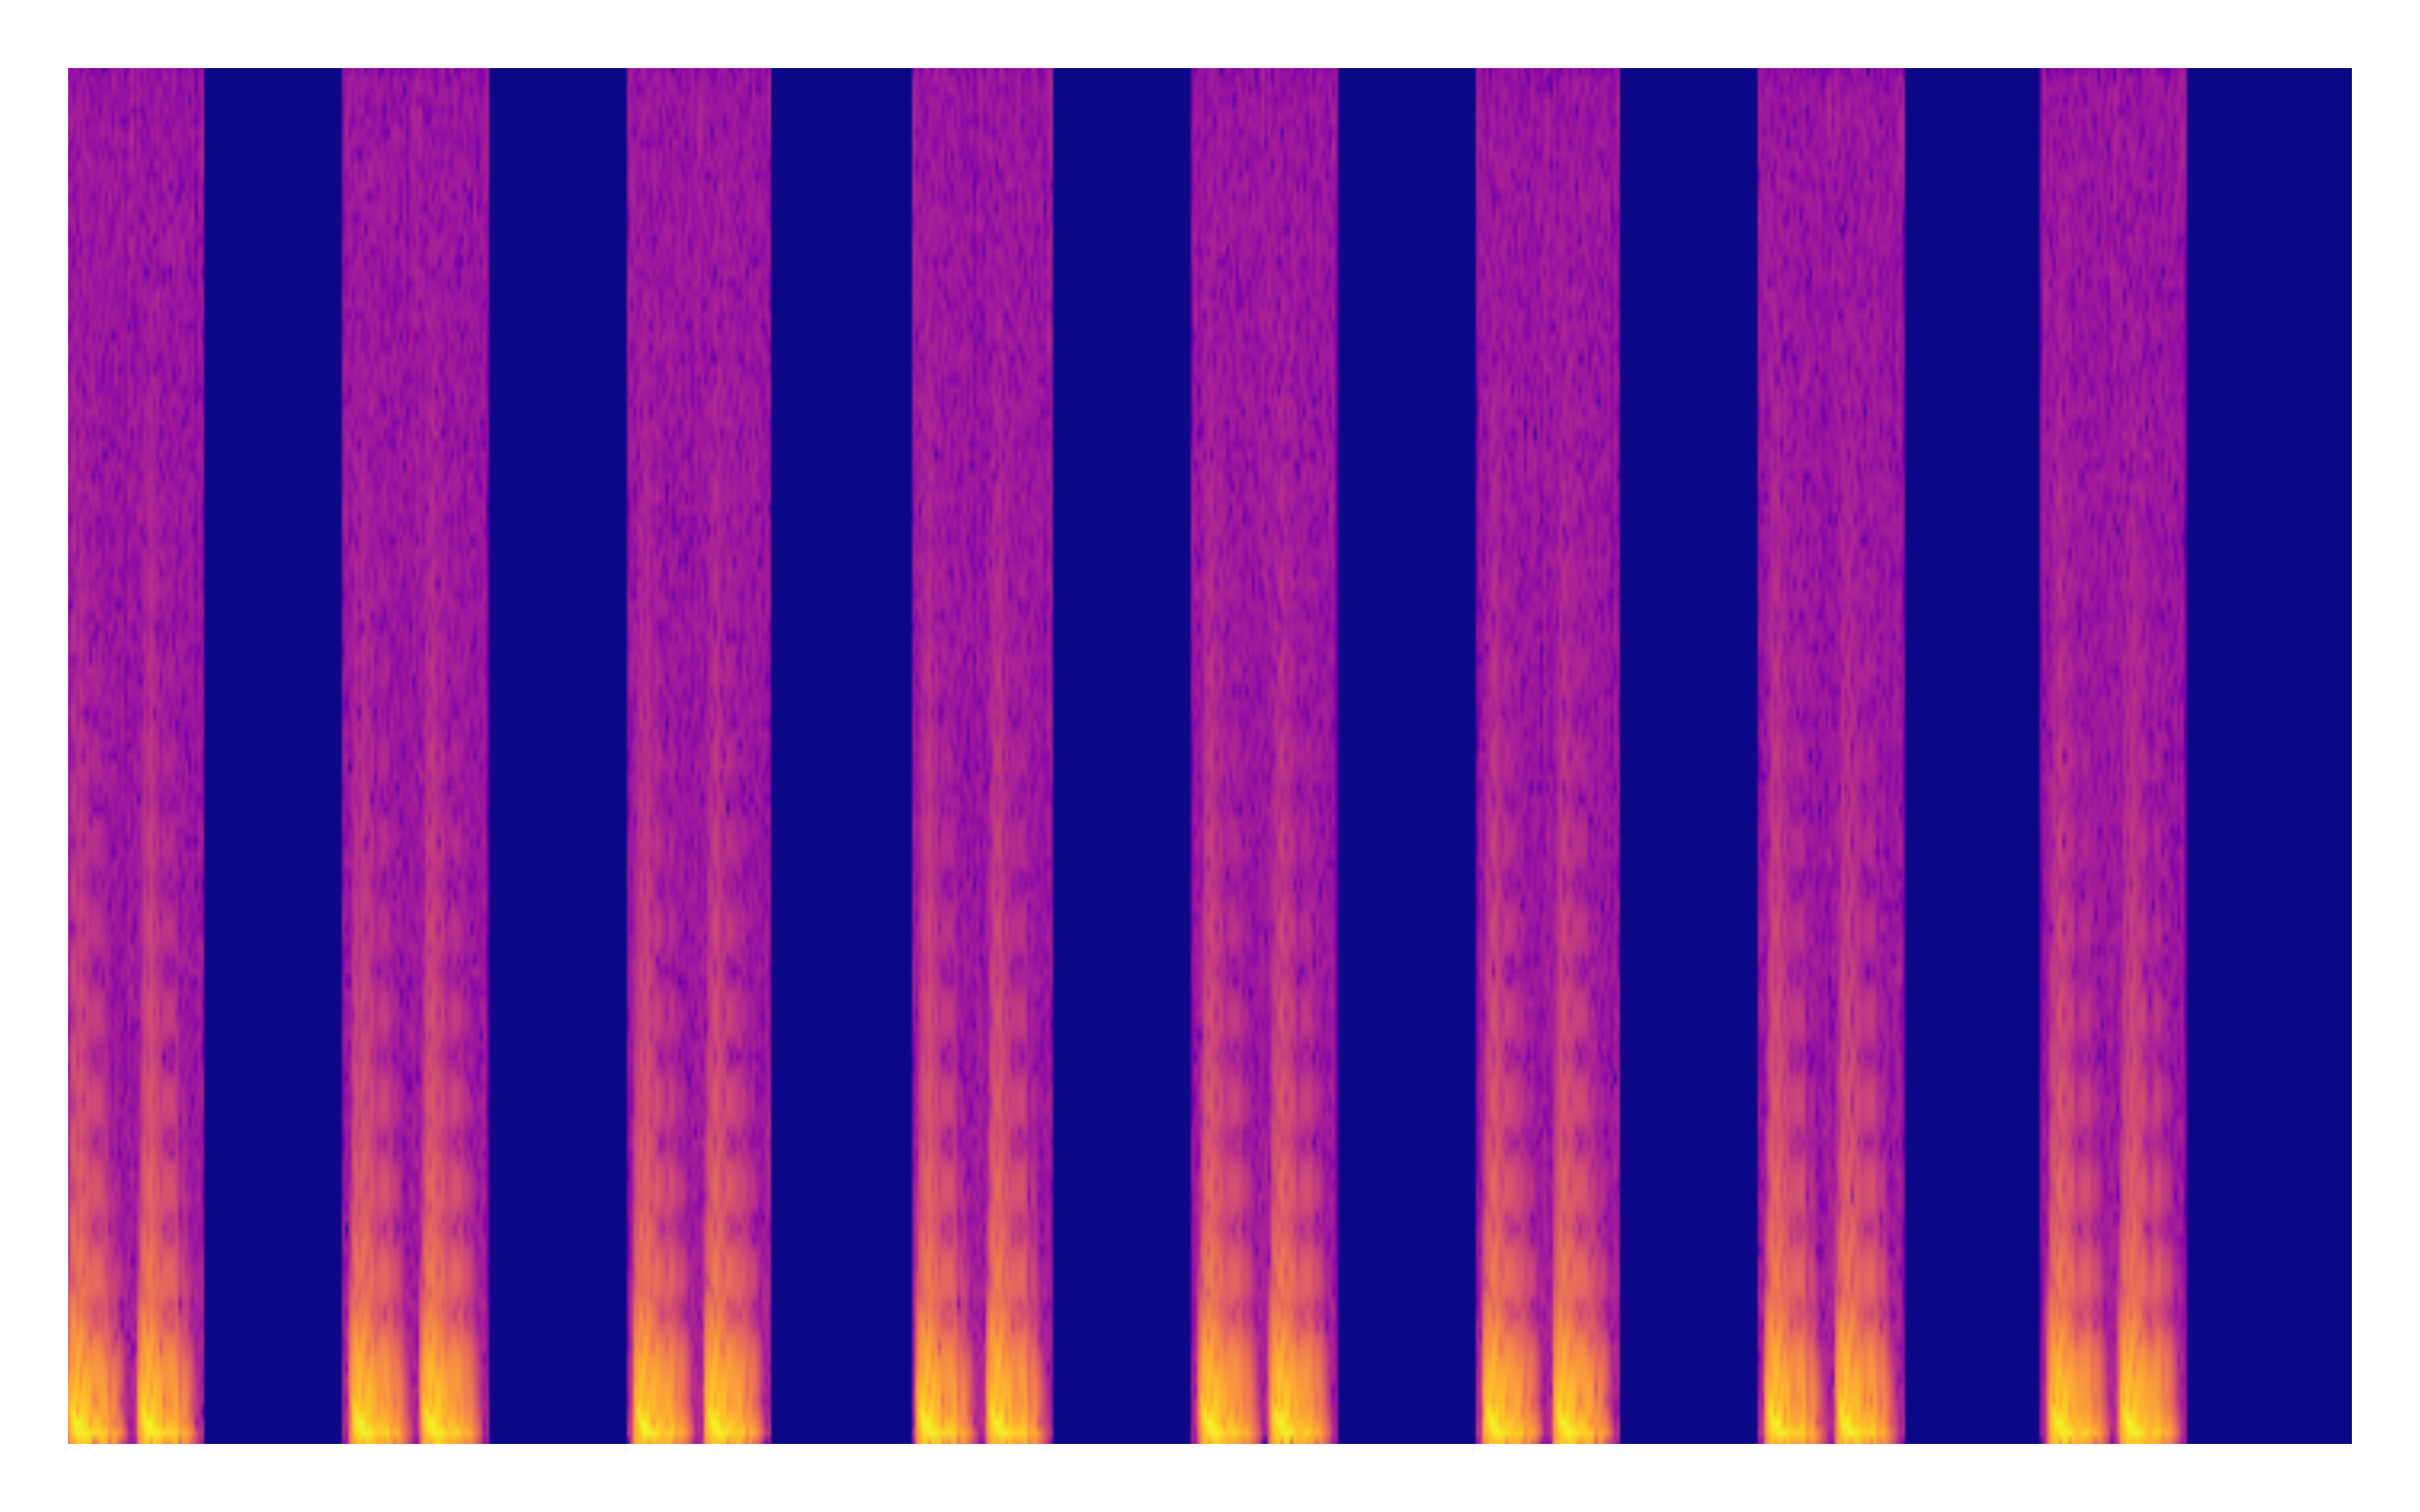
\includegraphics[width=\textwidth]{plots/onepeace_best_sdr/onepeace target_spectrogram.png}
    \end{subfigure}

    % Row 2 Best One-PEACE SDRi
    \begin{subfigure}[b]{0.185\textwidth}
        \centering
        \scriptsize\textbf{"Someone is shoveling something, making a clinking sound"}
        \vspace{5.0mm}
    \end{subfigure}
    \begin{subfigure}[b]{0.185\textwidth}
        \centering
        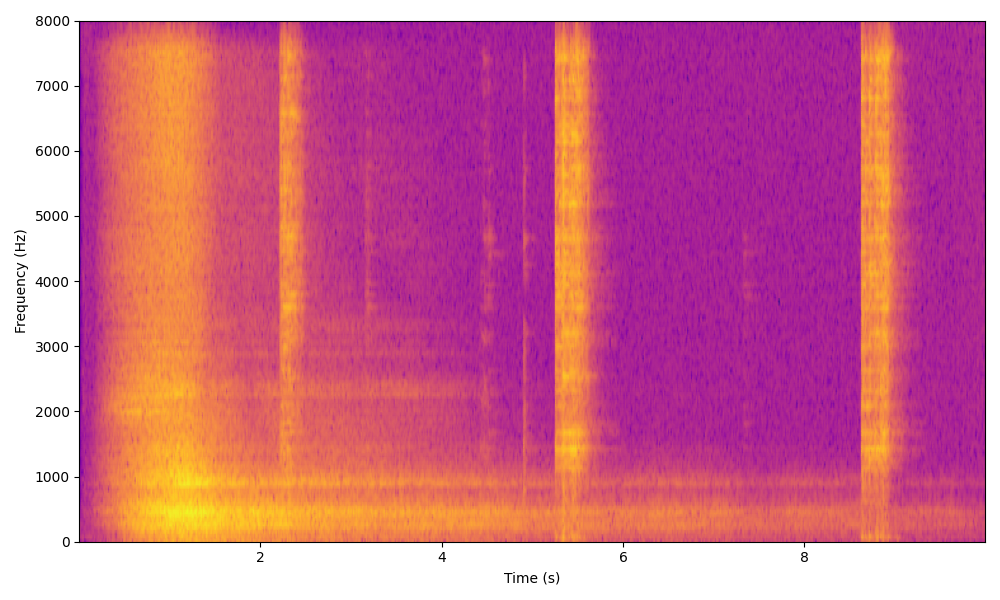
\includegraphics[width=\textwidth]{plots/onepeace_best_sdri/onepeace mixture_spectrogram.png}
    \end{subfigure}
    \begin{subfigure}[b]{0.185\textwidth}
        \centering
        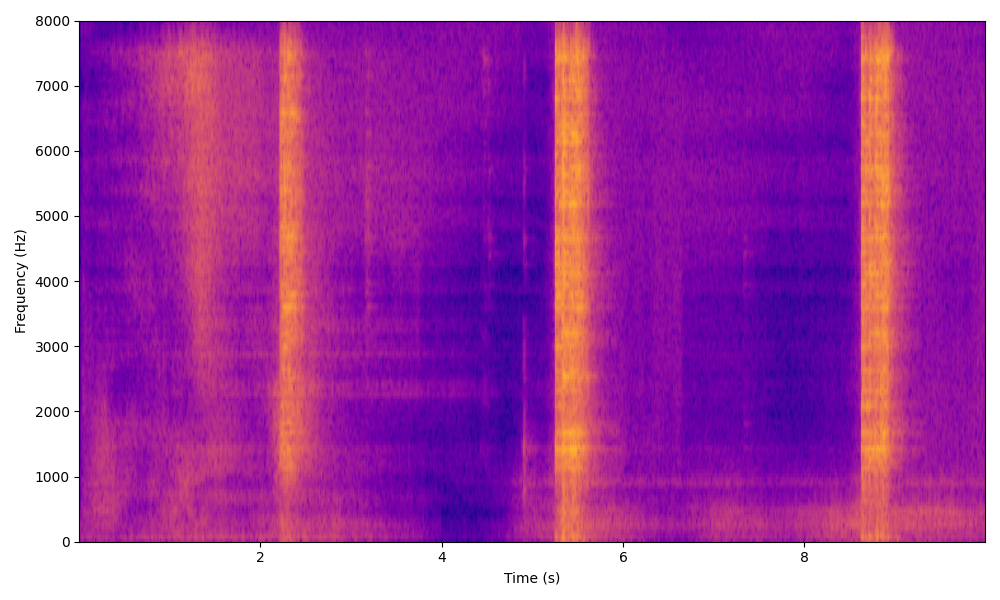
\includegraphics[width=\textwidth]{plots/onepeace_best_sdri/onepeace sep_spectrogram.png}
    \end{subfigure}
    \begin{subfigure}[b]{0.185\textwidth}
        \centering
        \includegraphics[width=\textwidth]{plots/onepeace_best_sdri/clap sep_spectrogram.png}
    \end{subfigure}
    \begin{subfigure}[b]{0.185\textwidth}
        \centering
        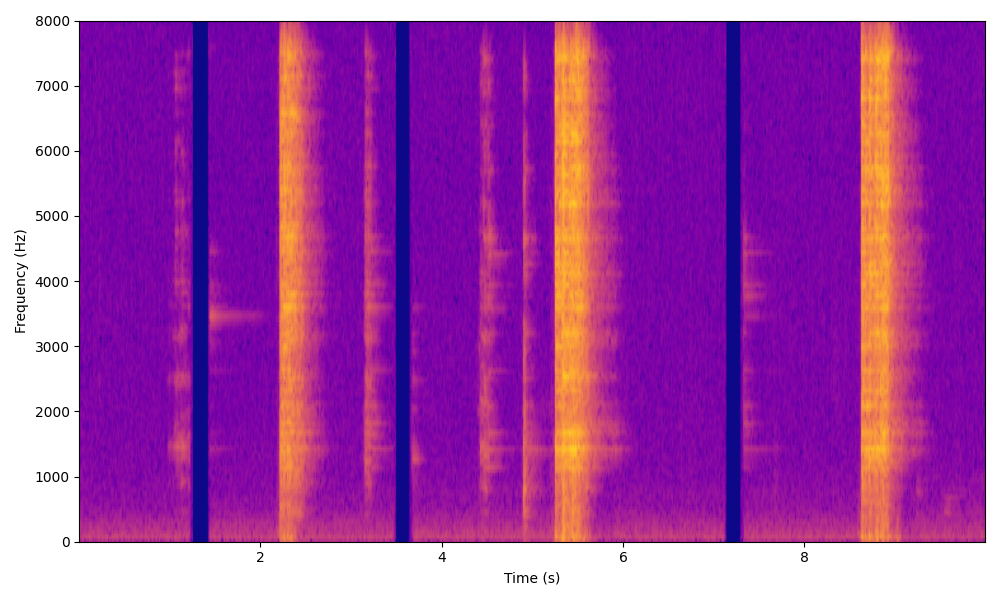
\includegraphics[width=\textwidth]{plots/onepeace_best_sdri/onepeace target_spectrogram.png}
    \end{subfigure}

    % Row 3 best onepeace delta_similarity improvement
     \begin{subfigure}[b]{0.185\textwidth}
        \centering
        \scriptsize\textbf{"Fireworks are shot into the air with swirling sounds and then they explode"}
        \vspace{5.0mm}
    \end{subfigure}
    \begin{subfigure}[b]{0.185\textwidth}
        \centering
        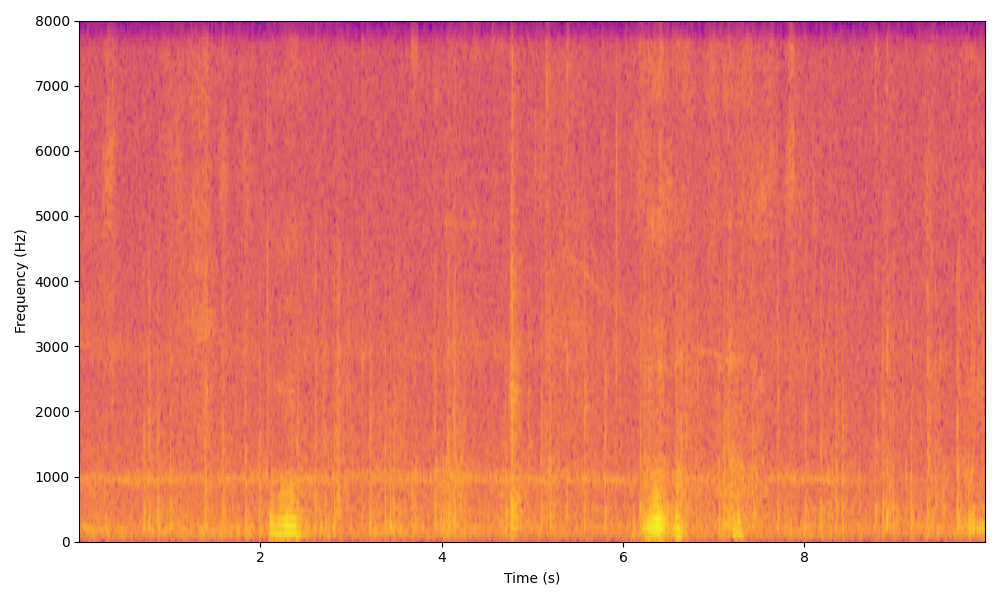
\includegraphics[width=\textwidth]{plots/onepeace_best_delta_similarity/onepeace mixture_spectrogram.png}
    \end{subfigure}
    \begin{subfigure}[b]{0.185\textwidth}
        \centering
        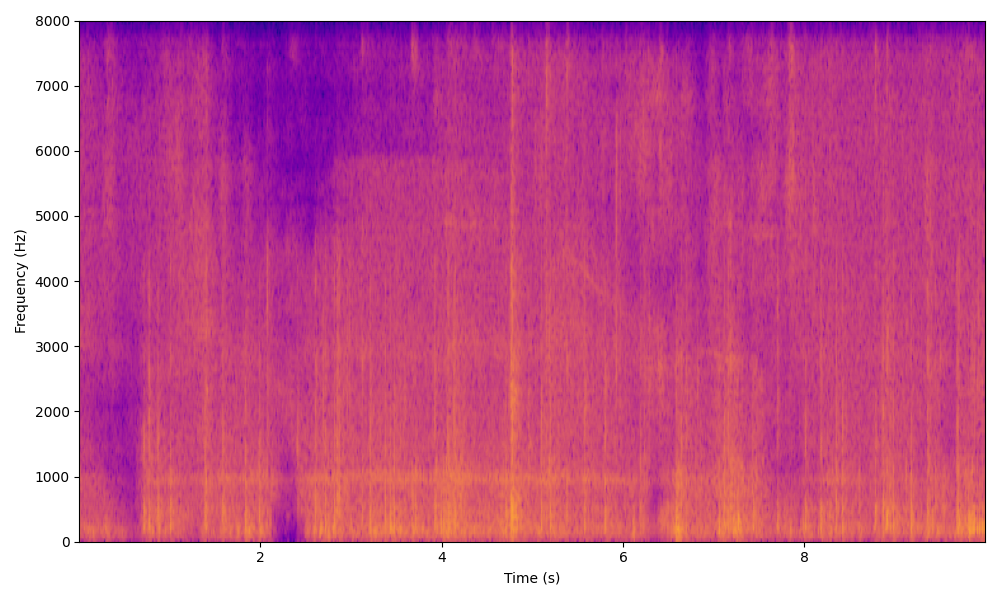
\includegraphics[width=\textwidth]{plots/onepeace_best_delta_similarity/onepeace sep_spectrogram.png}
    \end{subfigure}
    \begin{subfigure}[b]{0.185\textwidth}
        \centering
        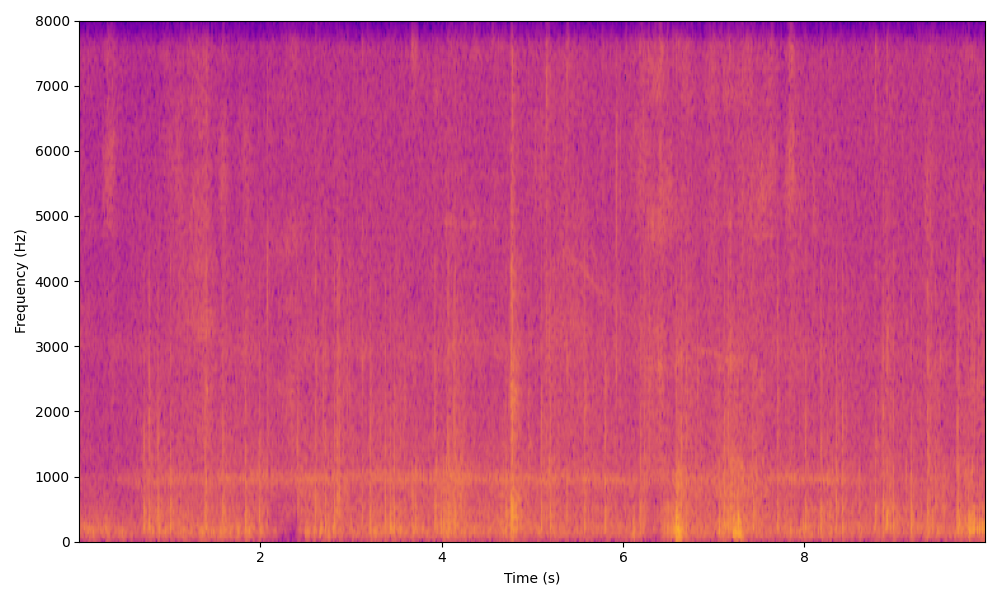
\includegraphics[width=\textwidth]{plots/onepeace_best_delta_similarity/clap sep_spectrogram.png}
    \end{subfigure}
    \begin{subfigure}[b]{0.185\textwidth}
        \centering
        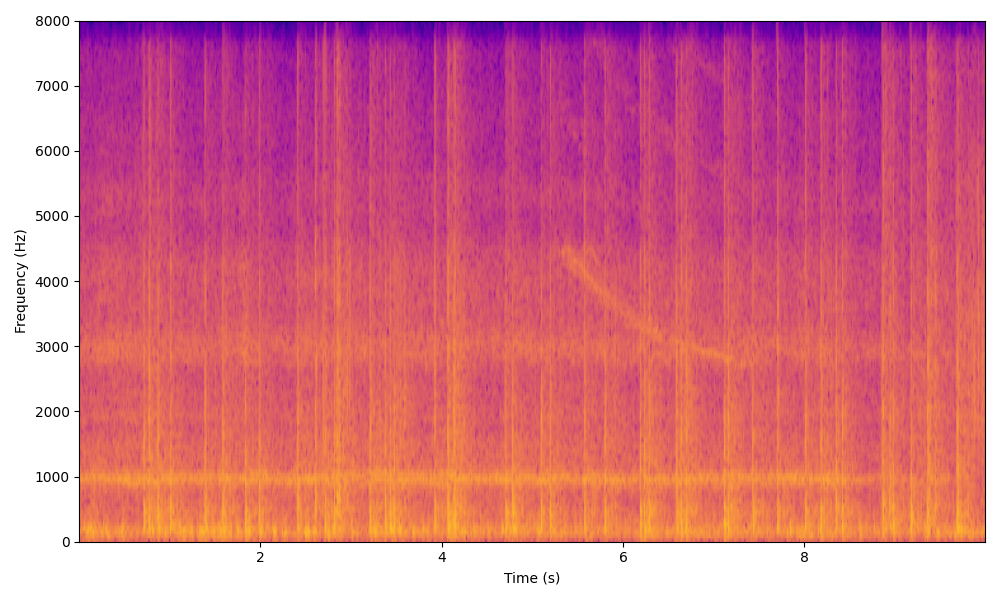
\includegraphics[width=\textwidth]{plots/onepeace_best_delta_similarity/onepeace target_spectrogram.png}
    \end{subfigure}
    
    
    % Row: high clap sdr, low onepeace sdr sword whoosh
    \begin{subfigure}[b]{0.185\textwidth}
        \centering
        \scriptsize\textbf{"The sword swooshes through the air as someone waves it, making a whooshing sound"}
        \vspace{5.0mm}
    \end{subfigure}
    \begin{subfigure}[b]{0.185\textwidth}
        \centering
        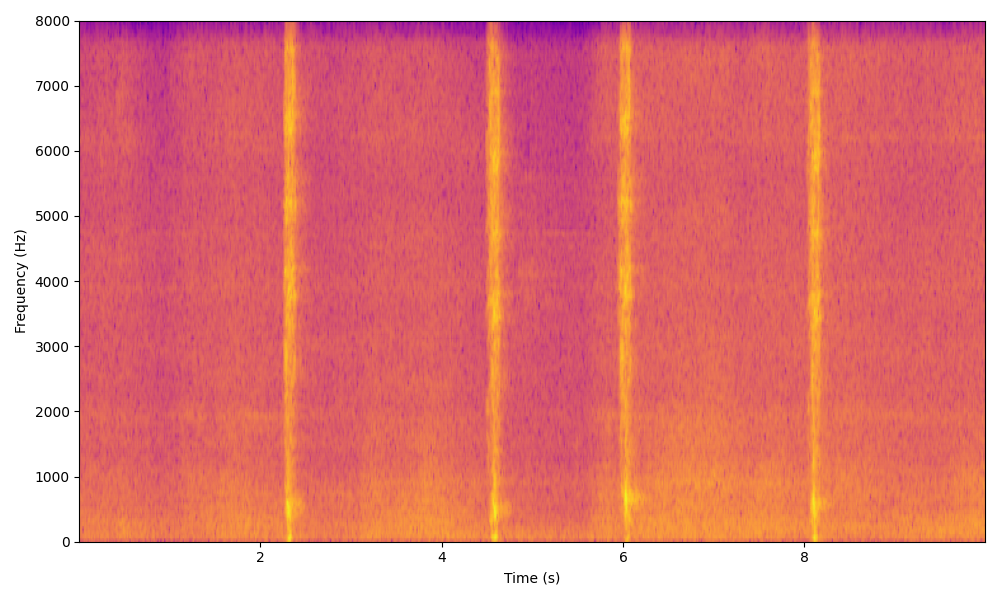
\includegraphics[width=\textwidth]{plots/sword_swoosh/clap mixture_spectrogram.png}
        \centering
    \end{subfigure}
    \begin{subfigure}[b]{0.185\textwidth}
        \centering
        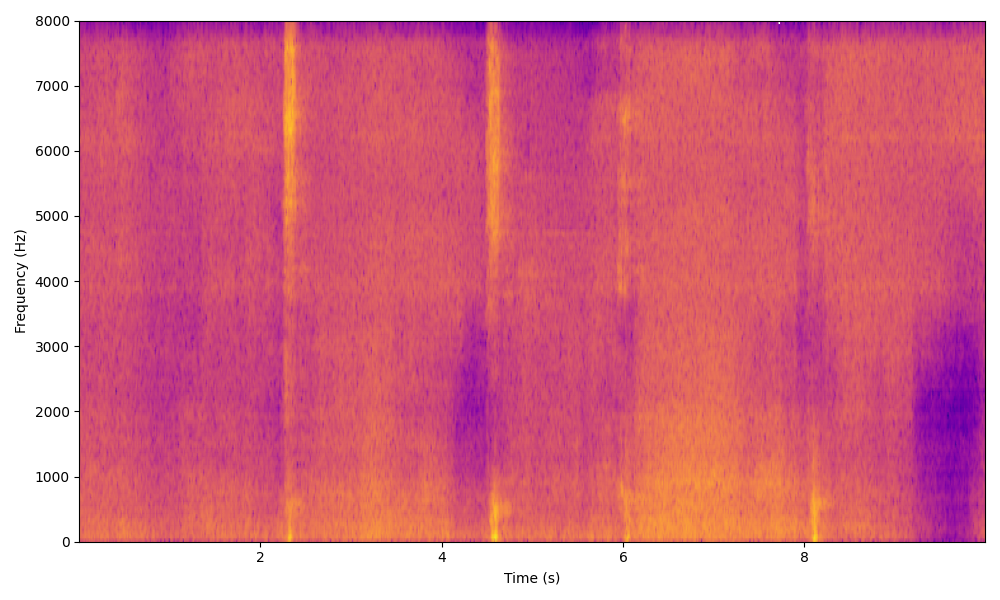
\includegraphics[width=\textwidth]{plots/sword_swoosh/onepeace sep_spectrogram.png}
    \end{subfigure}
    \begin{subfigure}[b]{0.185\textwidth}
        \centering
        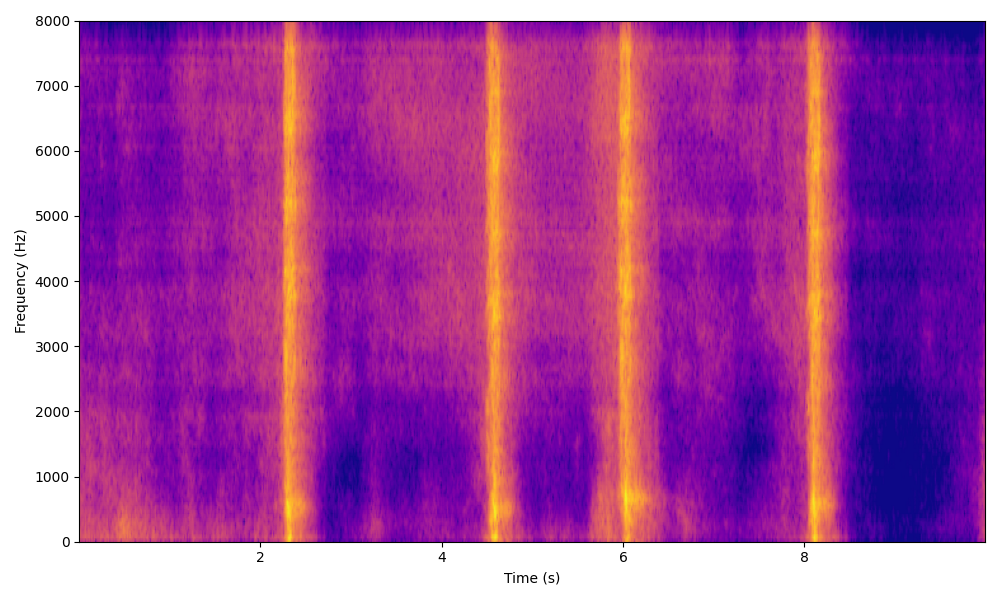
\includegraphics[width=\textwidth]{plots/sword_swoosh/clap sep_spectrogram.png}
    \end{subfigure}
    \begin{subfigure}[b]{0.185\textwidth}
        \centering
        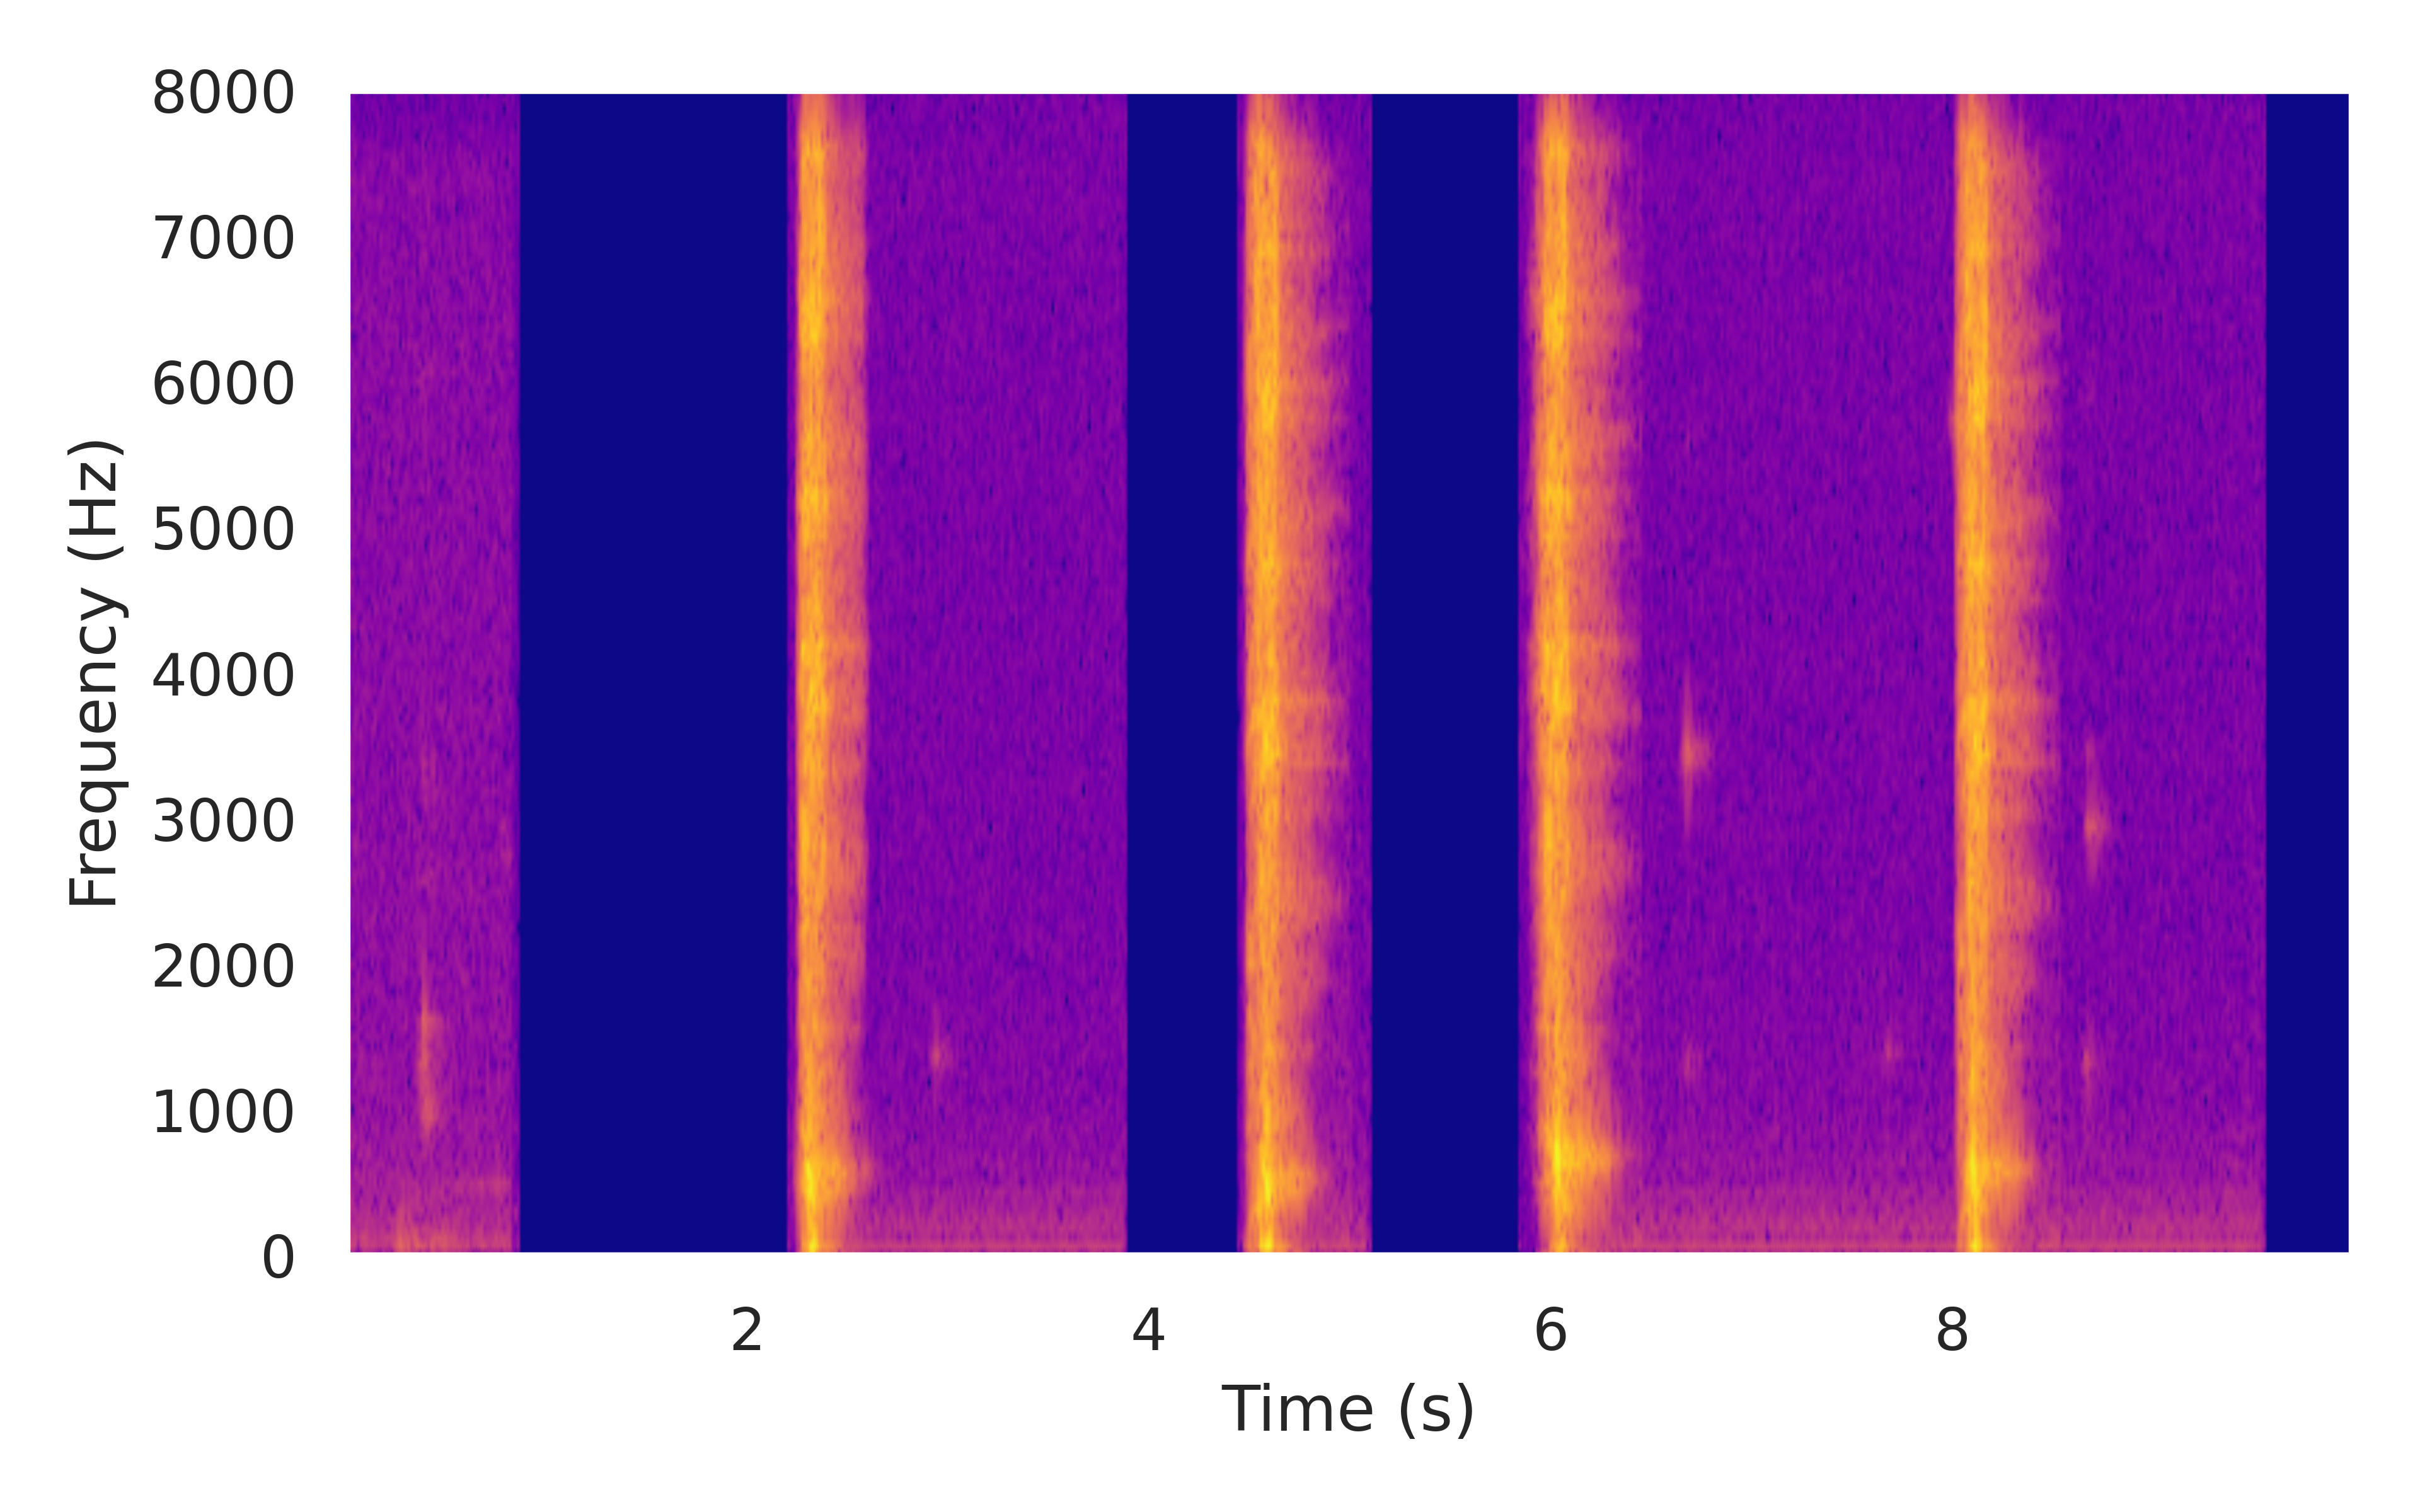
\includegraphics[width=\textwidth]{plots/sword_swoosh/clap target_spectrogram.png}
    \end{subfigure}

    % Row: high clap sdr, low onepeace sdr woosh_sound
    \begin{subfigure}[b]{0.185\textwidth}
        \centering
        \scriptsize\textbf{"A whooshing sound is moving rapidly"}
        \vspace{5.0mm}
        \caption*{Language Query}
    \end{subfigure}
    \begin{subfigure}[b]{0.185\textwidth}
        \centering
        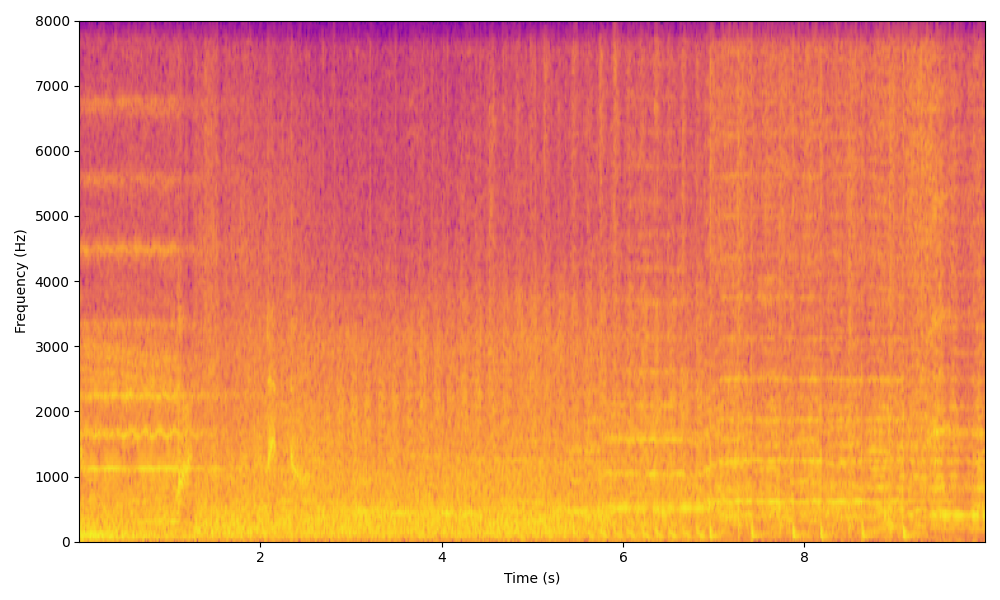
\includegraphics[width=\textwidth]{plots/whooshing_sound/clap mixture_spectrogram.png}
        \centering
        \caption*{Mixture}
    \end{subfigure}
    \begin{subfigure}[b]{0.185\textwidth}
        \centering
        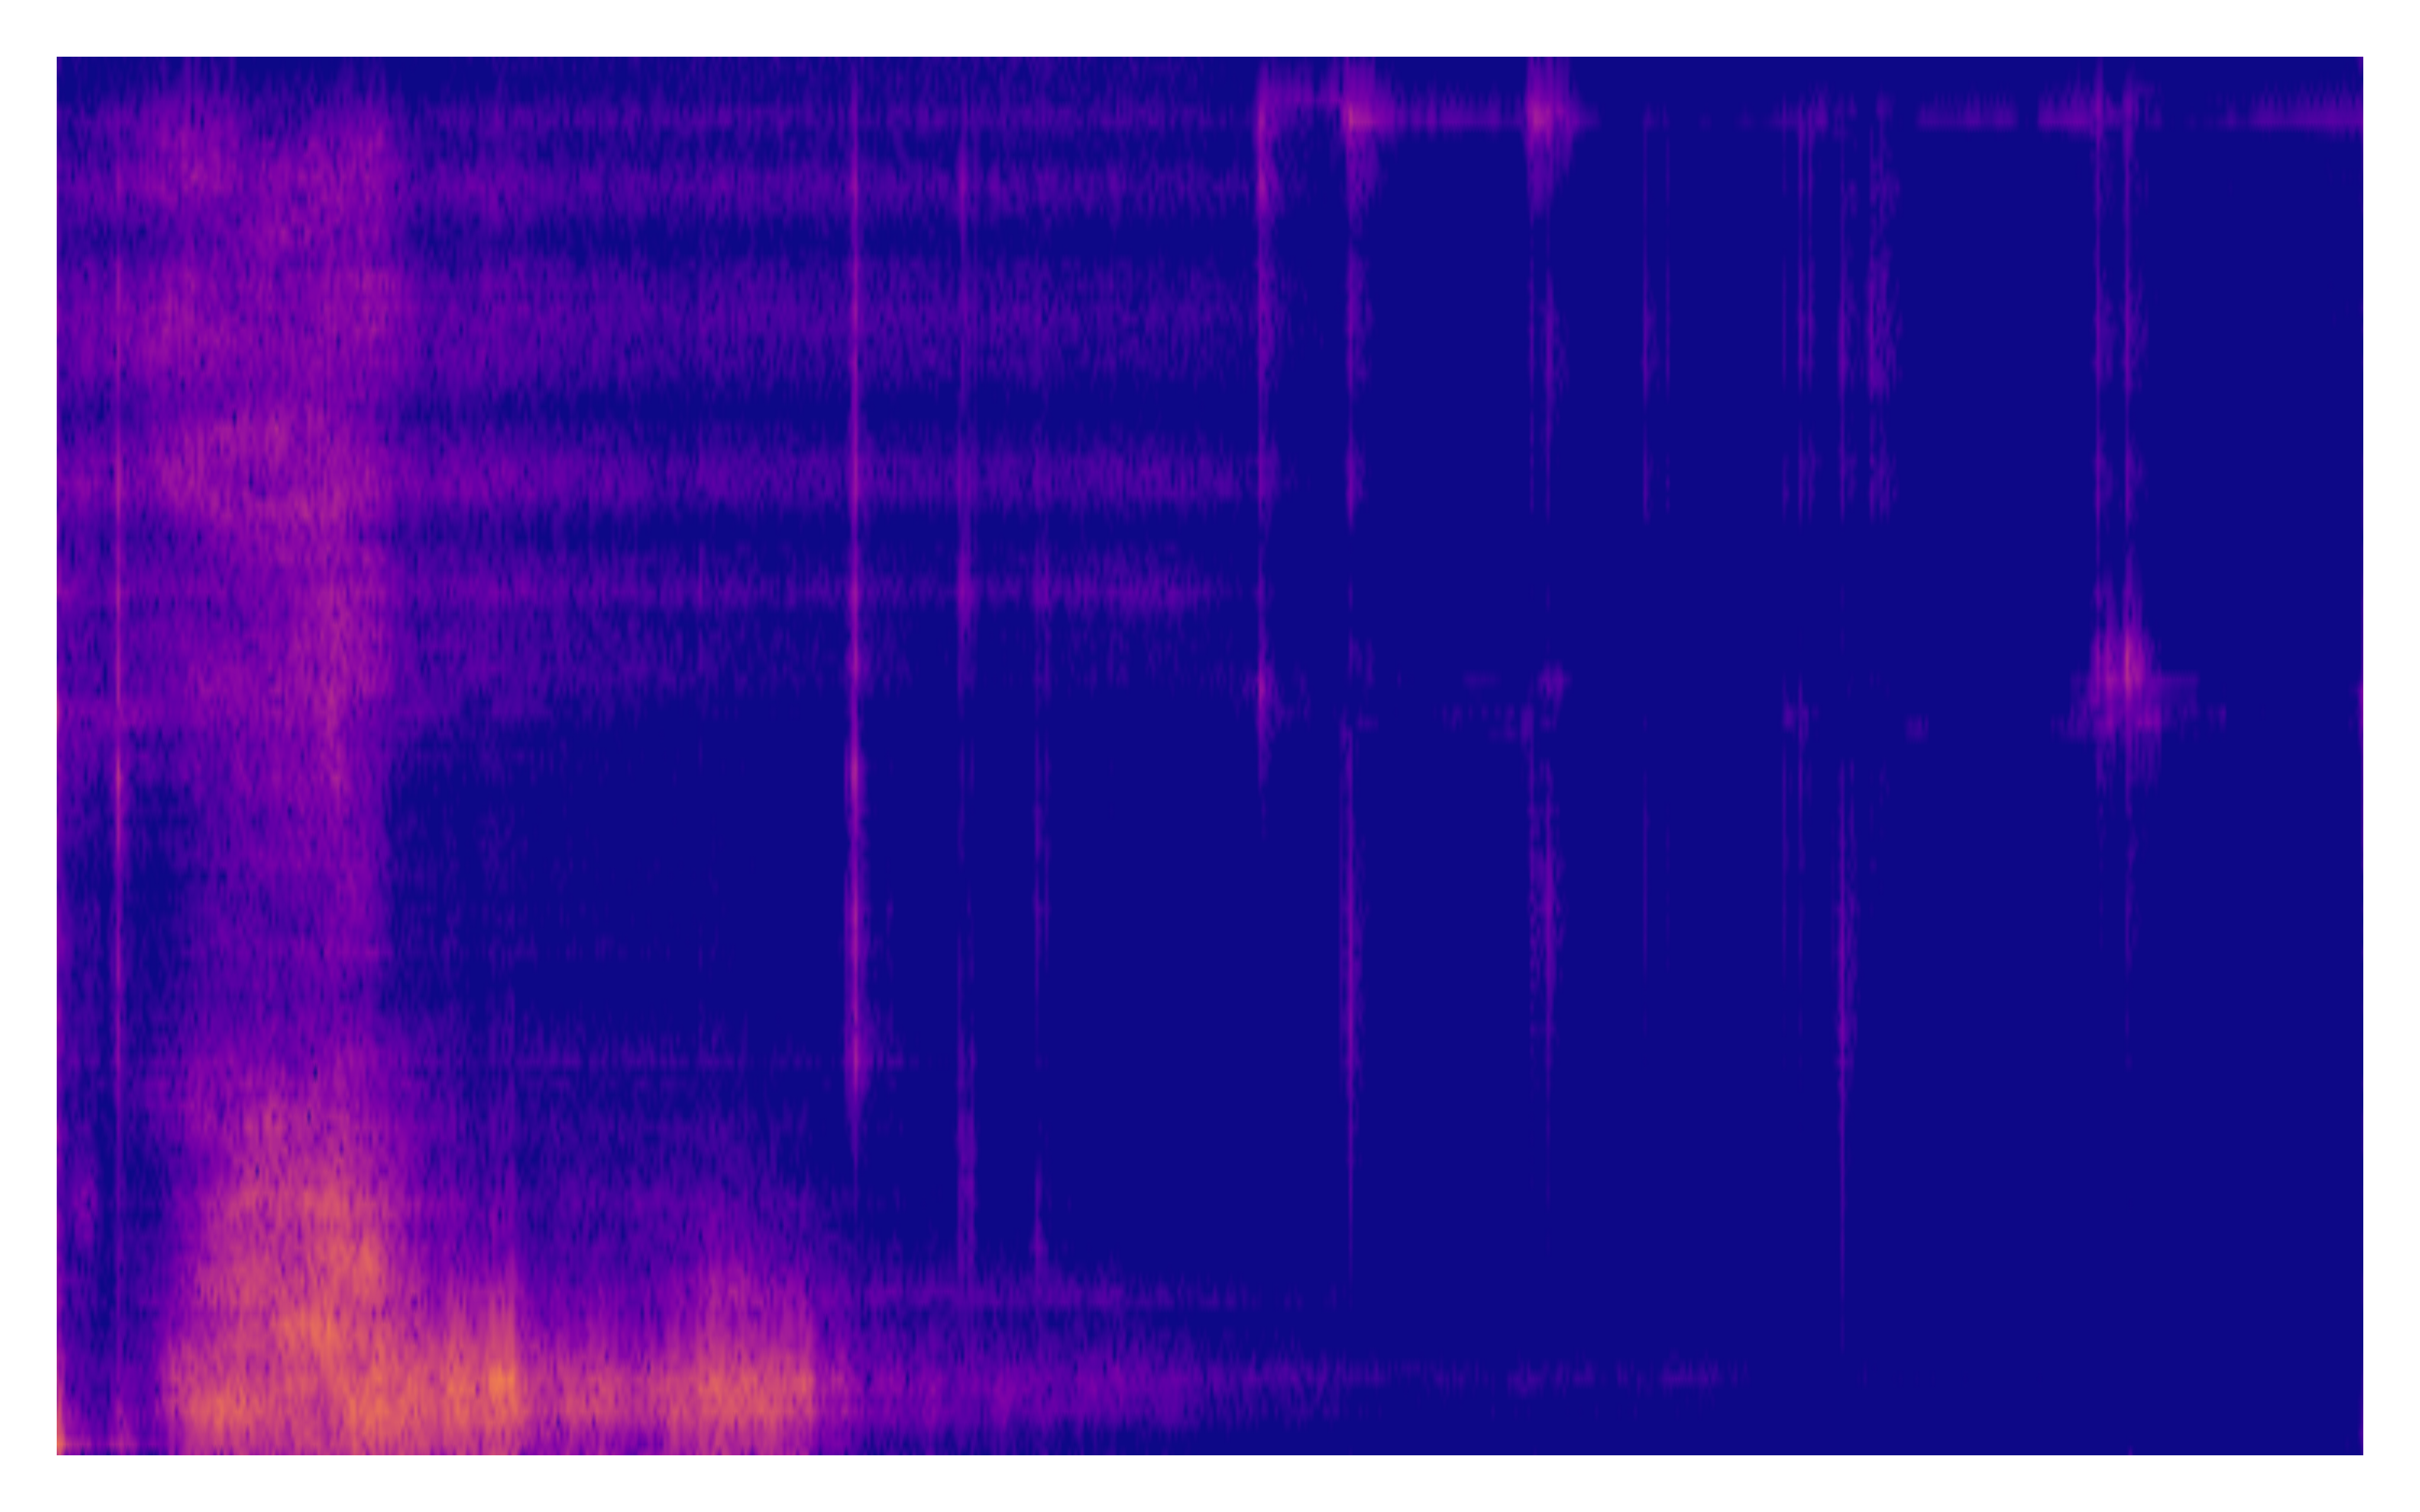
\includegraphics[width=\textwidth]{plots/whooshing_sound/onepeace sep_spectrogram.png}
        \caption*{One-Peace}
    \end{subfigure}
    \begin{subfigure}[b]{0.185\textwidth}
        \centering
        \includegraphics[width=\textwidth]{plots/whooshing_sound/clap sep_spectrogram.png}
        \caption*{CLAP}
    \end{subfigure}
    \begin{subfigure}[b]{0.185\textwidth}
        \centering
        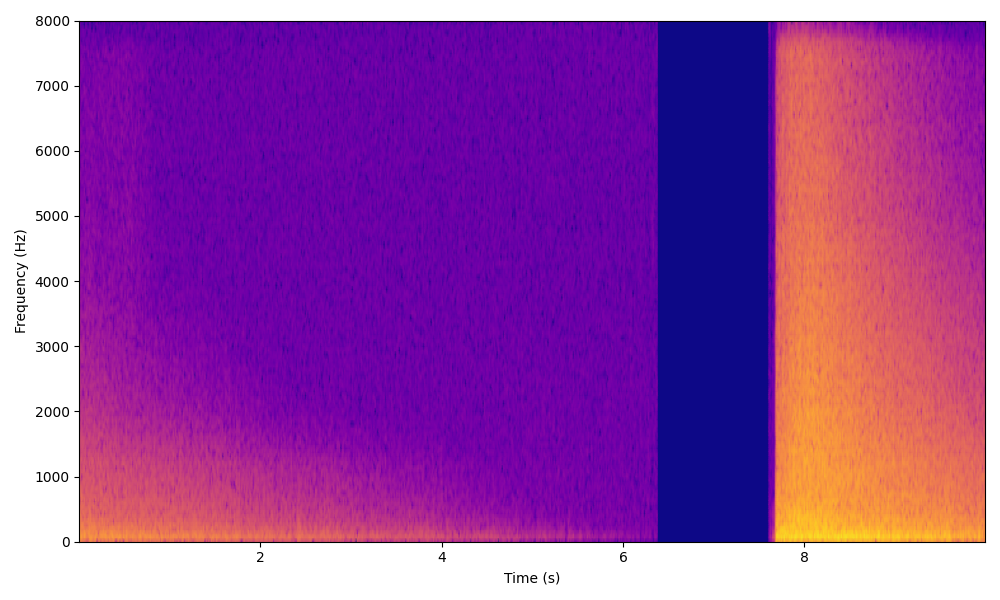
\includegraphics[width=\textwidth]{plots/whooshing_sound/clap target_spectrogram.png}
        \caption*{Target}
    \end{subfigure}
    
    % Continue rows similarly for other queries
    % Add caption below
    \caption{Visualized spectrograms for various language queries}
    
    \label{fig:separation_results}

\end{figure*}


\begin{table*}[ht]
\centering
\label{tab:audio_text_retrieval}
    \begin{tabular}{lcccccccccccc}
        \toprule
        \multirow{2}{*}{Method} & \multicolumn{6}{c}{AudioCaps} & \multicolumn{6}{c}{Clotho} \\
        \cmidrule(lr){2-7} \cmidrule(lr){8-13}
         & \multicolumn{3}{c}{Text $\to$ Audio} & \multicolumn{3}{c}{Audio $\to$ Text} & \multicolumn{3}{c}{Text $\to$ Audio} & \multicolumn{3}{c}{Audio $\to$ Text} \\
        \cmidrule(lr){2-4} \cmidrule(lr){5-7} \cmidrule(lr){8-10} \cmidrule(lr){11-13}
         & R@1 & R@5 & R@10 & R@1 & R@5 & R@10 & R@1 & R@5 & R@10 & R@1 & R@5 & R@10 \\
        \midrule

        % NOTE: taken from a table from the CLAP paper that isn't technically our checkpoint
        \textbf{CLAP} & 36.7 & 70.9 & 83.2 & 45.3 & 78.0 & 87.7 & 12.0 & 31.6 & 43.9 & 15.7 & 36.9 & 51.3 \\

        
        \textbf{ONE-PEACE} & \textbf{42.5} & \textbf{77.5} & \textbf{88.4} & \textbf{51.0} & \textbf{81.9} & \textbf{92.0} & \textbf{22.4} & \textbf{49.0} & \textbf{62.7} & \textbf{27.1} & \textbf{52.3} & \textbf{65.4} \\
        \bottomrule
    \end{tabular}
    
    \caption{Comparison of audio-text retrieval performance, taken from the CLAP and ONE-PEACE papers}
\end{table*}


\begin{table*}
  \centering
  \begin{tabular}{cccc}
                               & \multicolumn{3}{c}{\textbf{Number of Parameters}} \\
    \cline{2-4}
    % TODO: try to fix this to be a bit smaller
    \vspace{0.25mm} \\  
    \textbf{Model}             & \textbf{QueryNet}  & \textbf{SeparationNet} & \textbf{Total} \\
    \hline
    AudioSep-CLAP              &  199 M             &  29.6 M                & 229 M          \\
    AudioSep-ONE-PEACE\_al     &  2.75 B            &  39.7 M                & 2.79 B         \\
    AudioSep-ONE-PEACE\_full   &  4.00  B           &  39.7 M                & 4.04 B         \\
    \hline
  \end{tabular}
  \caption{Comparison of model sizes in our study}
\end{table*}
\todo[inline]{ONE-PEACE can be disassembled into different branches to handle different tasks, so the audio-language retrieval checkpoint is missing the image branch which makes it smaller}

\section{Engines}

To produce a PDF file, pdf\LaTeX{} is strongly recommended (over original \LaTeX{} plus dvips+ps2pdf or dvipdf). Xe\LaTeX{} also produces PDF files, and is especially suitable for text in non-Latin scripts.

% \section{Preamble}

% The first line of the file must be
% \begin{quote}
% \begin{verbatim}
% \documentclass[11pt]{article}
% \end{verbatim}
% \end{quote}

% To load the style file in the review version:
% \begin{quote}
% \begin{verbatim}
% \usepackage[review]{acl}
% \end{verbatim}
% \end{quote}
% For the final version, omit the \verb|review| option:
% \begin{quote}
% \begin{verbatim}
% \usepackage{acl}
% \end{verbatim}
% \end{quote}

% To use Times Roman, put the following in the preamble:
% \begin{quote}
% \begin{verbatim}
% \usepackage{times}
% \end{verbatim}
% \end{quote}
% (Alternatives like txfonts or newtx are also acceptable.)

% Please see the \LaTeX{} source of this document for comments on other packages that may be useful.

% Set the title and author using \verb|\title| and \verb|\author|. Within the author list, format multiple authors using \verb|\and| and \verb|\And| and \verb|\AND|; please see the \LaTeX{} source for examples.

% By default, the box containing the title and author names is set to the minimum of 5 cm. If you need more space, include the following in the preamble:
% \begin{quote}
% \begin{verbatim}
% \setlength\titlebox{<dim>}
% \end{verbatim}
% \end{quote}
% where \verb|<dim>| is replaced with a length. Do not set this length smaller than 5 cm.

\section{Document Body}

\subsection{Footnotes}

Footnotes are inserted with the \verb|\footnote| command.\footnote{This is a footnote.}

\subsection{Tables and figures}

See Table~\ref{tab:accents} for an example of a table and its caption.
\textbf{Do not override the default caption sizes.}

\begin{table}
  \centering
  \begin{tabular}{lc}
    \hline
    \textbf{Command} & \textbf{Output} \\
    \hline
    \verb|{\"a}|     & {\"a}           \\
    \verb|{\^e}|     & {\^e}           \\
    \verb|{\`i}|     & {\`i}           \\
    \verb|{\.I}|     & {\.I}           \\
    \verb|{\o}|      & {\o}            \\
    \verb|{\'u}|     & {\'u}           \\
    \verb|{\aa}|     & {\aa}           \\\hline
  \end{tabular}
  \begin{tabular}{lc}
    \hline
    \textbf{Command} & \textbf{Output} \\
    \hline
    \verb|{\c c}|    & {\c c}          \\
    \verb|{\u g}|    & {\u g}          \\
    \verb|{\l}|      & {\l}            \\
    \verb|{\~n}|     & {\~n}           \\
    \verb|{\H o}|    & {\H o}          \\
    \verb|{\v r}|    & {\v r}          \\
    \verb|{\ss}|     & {\ss}           \\
    \hline
  \end{tabular}
  \caption{Example commands for accented characters, to be used in, \emph{e.g.}, Bib\TeX{} entries.}
  \label{tab:accents}
\end{table}

As much as possible, fonts in figures should conform
to the document fonts. See Figure~\ref{fig:experiments} for an example of a figure and its caption.

Using the \verb|graphicx| package graphics files can be included within figure
environment at an appropriate point within the text.
The \verb|graphicx| package supports various optional arguments to control the
appearance of the figure.
You must include it explicitly in the \LaTeX{} preamble (after the
\verb|\documentclass| declaration and before \verb|\begin{document}|) using
\verb|\usepackage{graphicx}|.

\begin{figure}[t]
  \includegraphics[width=\columnwidth]{example-image-golden}
  \caption{A figure with a caption that runs for more than one line.
    Example image is usually available through the \texttt{mwe} package
    without even mentioning it in the preamble.}
  \label{fig:experiments}
\end{figure}

\begin{figure*}[t]
  \includegraphics[width=0.48\linewidth]{example-image-a} \hfill
  \includegraphics[width=0.48\linewidth]{example-image-b}
  \caption {A minimal working example to demonstrate how to place
    two images side-by-side.}
\end{figure*}

\subsection{Hyperlinks}

Users of older versions of \LaTeX{} may encounter the following error during compilation:
\begin{quote}
\verb|\pdfendlink| ended up in different nesting level than \verb|\pdfstartlink|.
\end{quote}
This happens when pdf\LaTeX{} is used and a citation splits across a page boundary. The best way to fix this is to upgrade \LaTeX{} to 2018-12-01 or later.

\subsection{Citations}

\begin{table*}
  \centering
  \begin{tabular}{lll}
    \hline
    \textbf{Output}           & \textbf{natbib command} & \textbf{ACL only command} \\
    \hline
    \citep{Gusfield:97}       & \verb|\citep|           &                           \\
    \citealp{Gusfield:97}     & \verb|\citealp|         &                           \\
    \citet{Gusfield:97}       & \verb|\citet|           &                           \\
    \citeyearpar{Gusfield:97} & \verb|\citeyearpar|     &                           \\
    \citeposs{Gusfield:97}    &                         & \verb|\citeposs|          \\
    \hline
  \end{tabular}
  \caption{\label{citation-guide}
    Citation commands supported by the style file.
    The style is based on the natbib package and supports all natbib citation commands.
    It also supports commands defined in previous ACL style files for compatibility.
  }
\end{table*}

Table~\ref{citation-guide} shows the syntax supported by the style files.
We encourage you to use the natbib styles.
You can use the command \verb|\citet| (cite in text) to get ``author (year)'' citations, like this citation to a paper by \citet{Gusfield:97}.
You can use the command \verb|\citep| (cite in parentheses) to get ``(author, year)'' citations \citep{Gusfield:97}.
You can use the command \verb|\citealp| (alternative cite without parentheses) to get ``author, year'' citations, which is useful for using citations within parentheses (e.g. \citealp{Gusfield:97}).

A possessive citation can be made with the command \verb|\citeposs|.
This is not a standard natbib command, so it is generally not compatible
with other style files.

\subsection{References}

\nocite{Ando2005,andrew2007scalable,rasooli-tetrault-2015}

The \LaTeX{} and Bib\TeX{} style files provided roughly follow the American Psychological Association format.
If your own bib file is named \texttt{custom.bib}, then placing the following before any appendices in your \LaTeX{} file will generate the references section for you:
\begin{quote}
\begin{verbatim}
\bibliography{custom}
\end{verbatim}
\end{quote}

You can obtain the complete ACL Anthology as a Bib\TeX{} file from \url{https://aclweb.org/anthology/anthology.bib.gz}.
To include both the Anthology and your own .bib file, use the following instead of the above.
\begin{quote}
\begin{verbatim}
\bibliography{anthology,custom}
\end{verbatim}
\end{quote}

Please see Section~\ref{sec:bibtex} for information on preparing Bib\TeX{} files.

\subsection{Equations}

An example equation is shown below:
\begin{equation}
  \label{eq:example}
  A = \pi r^2
\end{equation}

Labels for equation numbers, sections, subsections, figures and tables
are all defined with the \verb|\label{label}| command and cross references
to them are made with the \verb|\ref{label}| command.

This an example cross-reference to Equation~\ref{eq:example}.

\subsection{Appendices}

Use \verb|\appendix| before any appendix section to switch the section numbering over to letters. See Appendix~\ref{sec:appendix} for an example.

\section{Bib\TeX{} Files}
\label{sec:bibtex}

Unicode cannot be used in Bib\TeX{} entries, and some ways of typing special characters can disrupt Bib\TeX's alphabetization. The recommended way of typing special characters is shown in Table~\ref{tab:accents}.

Please ensure that Bib\TeX{} records contain DOIs or URLs when possible, and for all the ACL materials that you reference.
Use the \verb|doi| field for DOIs and the \verb|url| field for URLs.
If a Bib\TeX{} entry has a URL or DOI field, the paper title in the references section will appear as a hyperlink to the paper, using the hyperref \LaTeX{} package.

\section*{Acknowledgments}

This document has been adapted
by Steven Bethard, Ryan Cotterell and Rui Yan
from the instructions for earlier ACL and NAACL proceedings, including those for
ACL 2019 by Douwe Kiela and Ivan Vuli\'{c},
NAACL 2019 by Stephanie Lukin and Alla Roskovskaya,
ACL 2018 by Shay Cohen, Kevin Gimpel, and Wei Lu,
NAACL 2018 by Margaret Mitchell and Stephanie Lukin,
Bib\TeX{} suggestions for (NA)ACL 2017/2018 from Jason Eisner,
ACL 2017 by Dan Gildea and Min-Yen Kan,
NAACL 2017 by Margaret Mitchell,
ACL 2012 by Maggie Li and Michael White,
ACL 2010 by Jing-Shin Chang and Philipp Koehn,
ACL 2008 by Johanna D. Moore, Simone Teufel, James Allan, and Sadaoki Furui,
ACL 2005 by Hwee Tou Ng and Kemal Oflazer,
ACL 2002 by Eugene Charniak and Dekang Lin,
and earlier ACL and EACL formats written by several people, including
John Chen, Henry S. Thompson and Donald Walker.
Additional elements were taken from the formatting instructions of the \emph{International Joint Conference on Artificial Intelligence} and the \emph{Conference on Computer Vision and Pattern Recognition}.
N
% Bibliography entries for the entire Anthology, followed by custom entries
%\bibliography{anthology,custom}
% Custom bibliography entries only
\bibliography{custom}

\appendix

\section{Example Appendix}
\label{sec:appendix}

This is an appendix.

\end{document}
